\section[FASES ESTUDO]{FASES DO ESTUDO}
\subsection[Coleta dos Dados]{\textbf{Coleta dos Dados}}
Os dados para o treinamento da RNA CMAC são dados cinemáticos, capturados através de \emph{motion capture}, utilizando-se de várias câmeras \emph{Qualisys Oqus MRI}, com marcadores passivos e pacote de software \emph(QTM 3.2) da \emph{Qualisys}. 
O sistema utilizado suporta até 74 canais, ou marcadores simultâneos.

O projeto no qual ocorreu a coleta foi aprovado pelo Comitê de Ética da Faculdade de Saúde da UnB, processo N11911/12 (ver Anexo \ref{anexo1}).

A Figura \ref{coleta_dados} mostra o processo para coleta de dados.

\begin{figure}[ht]
 \centering
 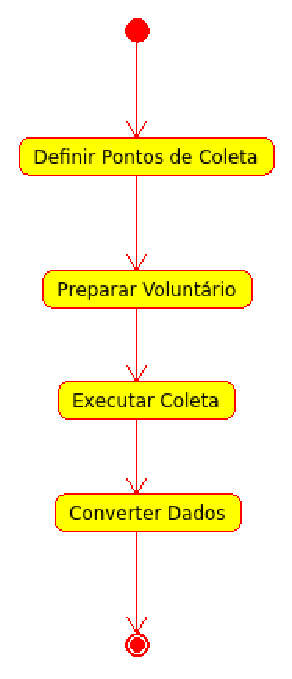
\includegraphics[width=4cm]{figuras/coleta_dados.eps}
 \caption{Fluxo de coleta de dados.}
 \label{coleta_dados}
\end{figure}

Primeiro deve-se definir o voluntário da coleta e determinar o dia para este processo. 
Além disso, também é necessário definir quais os pontos no corpo do voluntário devem ser mapeados. 
Também se devem distribuir os marcadores em várias posições ao longo das pernas. 
Como só a flexão e a extensão dos joelhos interessam para este trabalho, utilizam-se somente marcadores nas tíbias, joelhos e trocânteres das duas pernas.

O próximo passo se refere ao voluntário, isto é, ele deve repetir um ciclo de marcha confortável de aproximadamente 5 segundos, por 5 vezes na frente das câmeras.

Quanto aos dados, estes devem ser convertidos para formato adequado à linguagem \emph{Octave}, que é a mesma opção para converter para o \emph{MATLAB}. Esta opção é própria do \emph{QTM}. 
Além da conversão é necessário definir o nome de cada item na matriz de dados coletados. 
Cada coluna desta matriz representa um marcador, são estes pontos que devem ser nomeados. 
Por exemplo, coluna 1 igual ao trocânter direito. 
O número que o QTM atribui internamente ao marcador é a posição do marcador na matriz. 
Este número é chamado dentro do QTM de canal. 
Os dados trazem variáveis espaciais e o erro, com respeito à posição (X, Y, Z) dos marcadores.

A disposição que os dados obtidos neste processo se apresentam, é mostrado na Figura \ref{dados_qtm}.

\begin{figure}[ht]
 \centering
 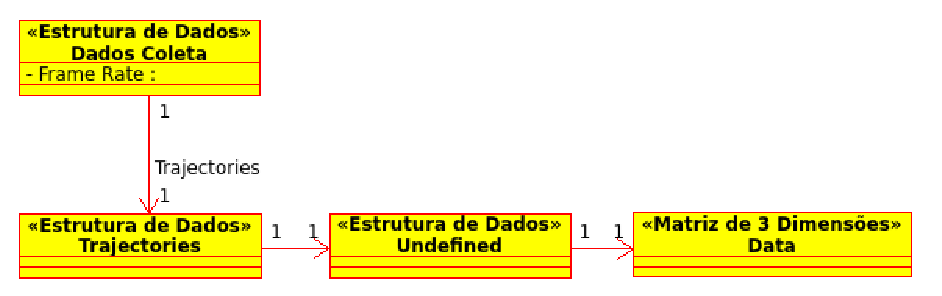
\includegraphics[width=15cm]{figuras/dados_qtm.eps}
 \caption{Dados disponibilizados pelo QTM.}
 \label{dados_qtm}
\end{figure}

Os dados que interessam são o \emph{Frame Rate} e o \emph{Data}.
São retornados vários dados, mas os de interesse para o projeto são os que estão na Figura \ref{dados_qtm}. 
O \emph{Frame Rate} é a taxa de coleta dos dados e está em segundos. 
A matriz de 3 dimensões está disposta da seguinte forma:
\begin{enumerate}
	\item A primeira dimensão é 74 e representa o número de canais do sistema de coleta;
	\item A segunda dimensão é 4 e representa a posição num plano 3D (X, Y, Z) do marcador, mais o erro;
	\item A terceira dimensão é número de frames coletados numa caminhada específica. Este número é variável.
\end{enumerate}



\subsection[Extração e transformação dos dados]{\textbf{Extração e transformação dos dados}}
Com os dados necessários disponibilizados no formato adequado é possível fazer os cálculos de angulações, velocidades angulares e acelerações angulares dos joelhos. Os casos de uso para esta fase são:
\begin{figure}[ht]
	\centering
	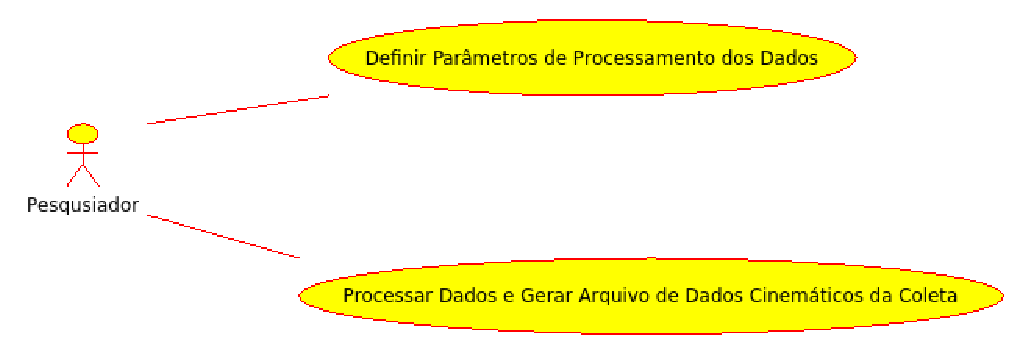
\includegraphics[width=15cm]{figuras/extracao_coleta.eps}
	\caption{Caso de uso para extração e transformação de dados}
	\label{extracao_coleta}
\end{figure}

O caso de uso Definir Parâmetros de Processamento dos Dados, definido na Figura \ref{extracao_coleta}, consiste em se definir os dados necessários para que depois seja possível processar os dados coletados. 
Estes dados são os definidos na Figura \ref{estrutura_dados}. 
O valor dos 6 primeiros atributos da estrutura de dados Configuração do Processamento, são os canais usados no QTM para tais marcadores.
\begin{figure}[ht]
	\centering
	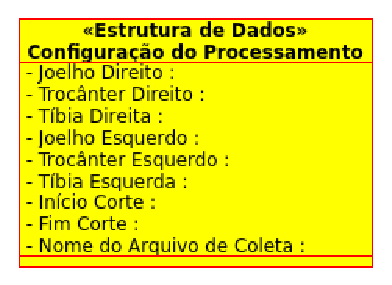
\includegraphics[width=7.5cm]{figuras/estrutura_dados.eps}
	\caption{Dados para processamento da coleta.}
	\label{estrutura_dados}
\end{figure}

O caso de uso Processar Dados e Gerar Arquivos de Dados Cinemáticos, definido na Figura \ref{extracao_coleta}, da coleta deve obedecer o processo da Figura \ref{tratamento_dados}.
\begin{figure}[ht]
	\centering
	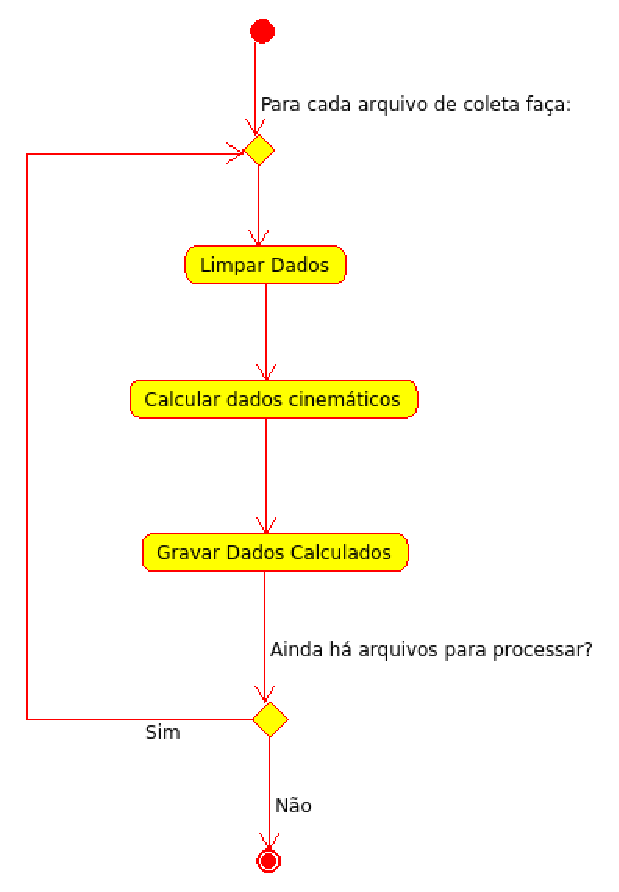
\includegraphics[width=10cm]{figuras/tratamento_dados.eps}
	\caption{Processo de tratamento dos dados.}
	\label{tratamento_dados}
\end{figure}

A limpeza dos dados consiste em retirar os dados desnecessários, como marcadores não desejados e retirada de frames do início e/ou final de um arquivo de coleta, que não estejam no ciclo de marcha confortável. 

Os cálculos realizados devem ser as velocidades instantâneas, velocidades angulares e acelerações angulares. 
Velocidades instantâneas dos joelhos são calculadas conforme a Equação \ref{velocidade}.
\begin{equation}
	\label{velocidade}
	\vec{\nu} = (\vec{a}-\vec{b})/t 
\end{equation}

A variável $\vec{a}$  é a posição (X, Y, Z) do joelho em uma determinada leitura sequencial dos dados coletados. 
A variável $\vec{b}$ é a próxima posição (X, Y, Z) da sequência. $t$ é o \emph{frame rate} definido nos dados da coleta.

Para o cálculo das angulações dos joelhos, primeiro os marcadores destes devem ser transladados para uma origem, assim é possível se usar a Equação 5 como descrita em \citeonline{Edwards2006}. 
Para tal, usam-se as Equações \ref{trocanter}, \ref{joelho} e \ref{tibia}.
\begin{equation}
	\label{trocanter}
	\vec{t_{r0}} = \vec{t_r} - \vec{j}
\end{equation}
\begin{equation}
	\label{joelho}
	\vec{j_0} = \vec{j} - \vec{j}
\end{equation}
\begin{equation}
	\label{tibia}
	\vec{t_{b0}} = \vec{t_b} - \vec{j}
\end{equation}

$\vec{t_{r0}}$ é o vetor que representa a posição de um trocânter $\vec{t_r}$, transladado para a nova origem.
$\vec{j}$ é vetor da posição do joelho.
$\vec{j_0}$ é a nova origem, que nada mas é que o joelho transladado para a posição $(0,0,0)$. 
$\vec{t_{b0}}$ é a posição da tíbia $\vec{t_b}$ transladada para a origem.
A translação de vetores é documentada em \citeonline{Poole2011}.

Agora que se tem os pontos transladados para uma origem, pode-se usar a Equação \ref{ang_joe} para o cálculo do ângulo $\theta$ do joelho.
\begin{equation}
	\label{ang_joe}
	\theta =
		cos^{-1} 
		\frac
		{
			\vec{t_{r0}} \cdot \vec{t_{b0}}
		}
		{
			\left \| \vec{t_{r0}} \right \|
			\cdot
			\left \| \vec{t_{b0}} \right \|
		}
\end{equation}

O operador $\left \| \right \|$ é o cálculo da distância euclidiana, ou norma. Pode ser calculado, segundo \citeonline{Poole2011}, de acordo com a Equação \ref{norma}. Resumindo, é a raiz quadrada do produto interno de um vetor.
\begin{equation}
	\label{norma}
	\left \| \vec{u} \right \| = \sqrt{\vec{u}\cdot\vec{u}}
\end{equation}

A velocidade angular $\omega$ do joelho é calculada a partir da Equação \ref{vel_ang}.
\begin{equation}
	\label{vel_ang}
	\omega = (\theta_1 - \theta_2) / t
\end{equation}

A variável $\theta_1$ é o ângulo de um joelho num determinado frame. A variável $\theta_2$ é exatamente o ângulo do próximo frame. A variável $t$ é o \emph{frame rate}, oriundo dos dados da coleta.


A última etapa deste processo é a gravação dos dados para que possam ser usados pela RNA CMAC. 
Estes dados devem ser gravados num arquivo em formato texto. 
As linhas neste arquivo equivalem aos \emph{frames}. 
Cada coluna equivale às informações, na ordem em que aparecem, da estrutura de dados descrita na Figura \ref{dados_cinematicos}. 
\begin{figure}[ht]
	\centering
	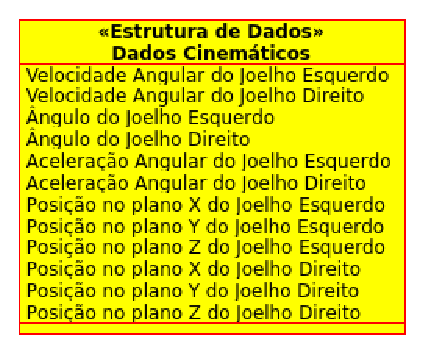
\includegraphics[width=7.5cm]{figuras/dados_cinematicos.eps}
	\caption{Dados Cinemáticos da Marcha}
	\label{dados_cinematicos}
\end{figure}

\subsection[Construção de uma RNA CMAC]{\textbf{Construção}}
\subsubsection{Modelo Geral}

A RNA CMAC proposta para este trabalho é resumida na Figura \ref{camac_resumida}.

\begin{figure}[ht]
	\centering
	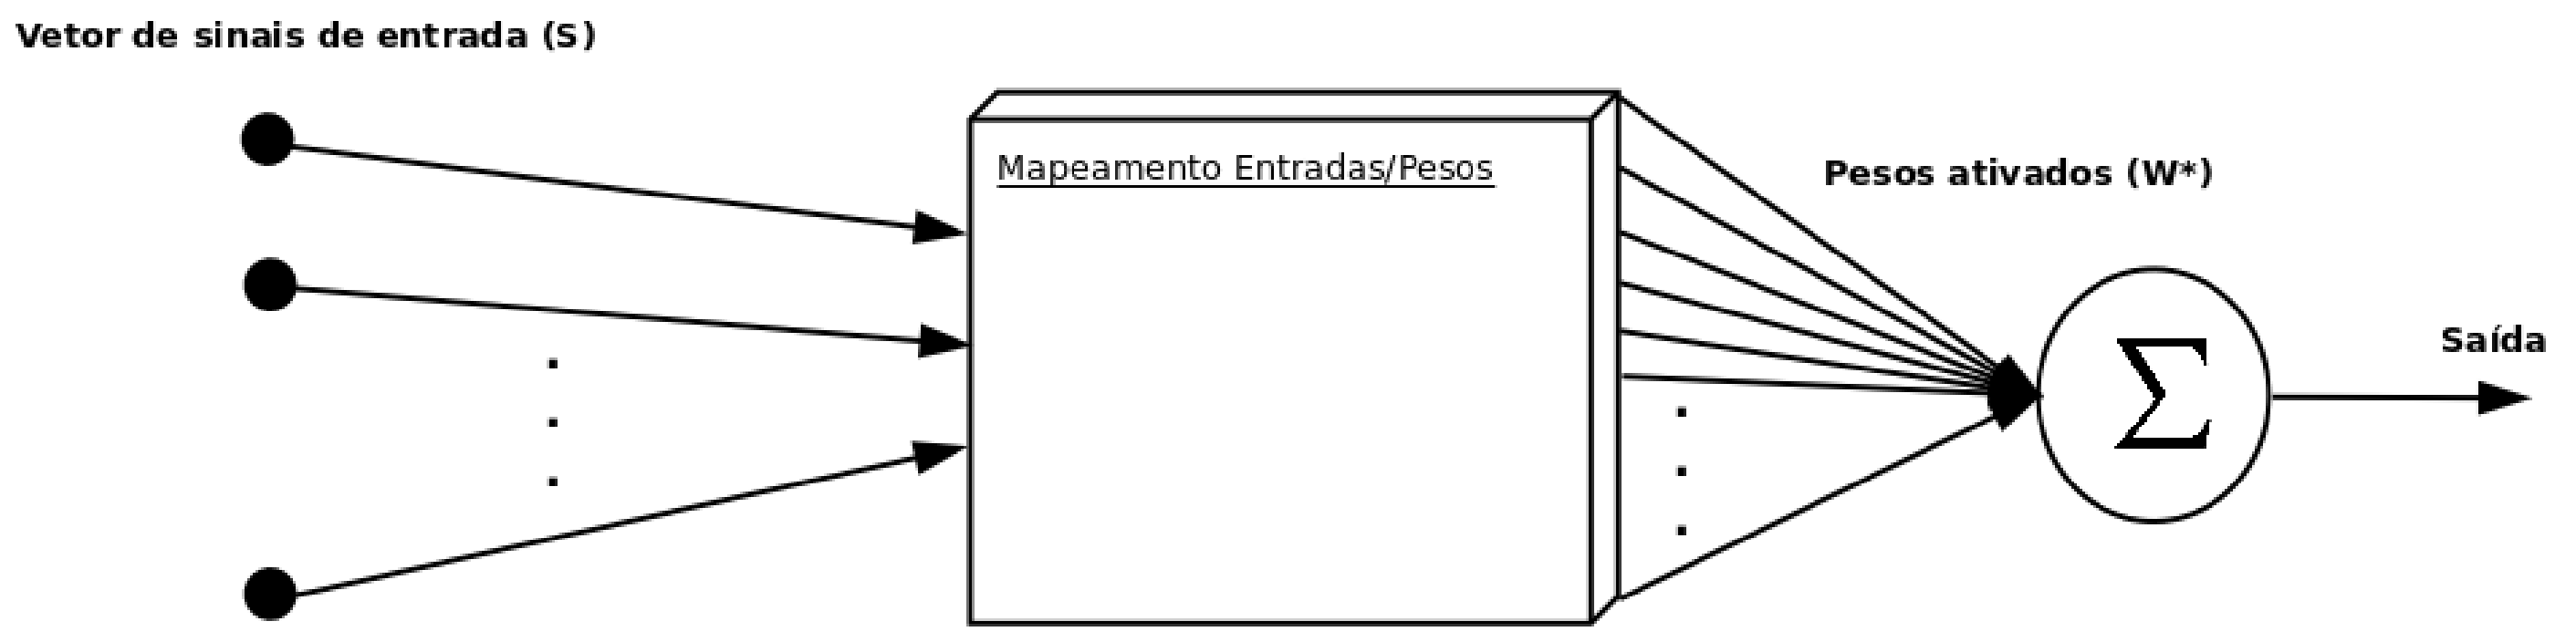
\includegraphics[width=15cm]{figuras/cmac_resumida.eps}
	\caption{CMAC resumida.}
	\label{camac_resumida}
\end{figure}

A variável $S$ é o vetor de sinais de entrada. 
Esses sinais são passados para um processo de mapeamento entre a entrada e um conjunto de pesos. 
Depois apenas os pesos ativados participam da somatória que é o sinal de saída. 

Para se calcular a saída da rede, primeiramente define-se o número de pesos $NW*$ a serem ativados.

O segundo passo é definir os possíveis valores para cada item do vetor de entradas $S$. A isto chama-se quantização. Por exemplo, se o primeiro item $s1$ de $S$ aceita valores entre $-1$ até $1$ e se quer $5$ valores possíveis, quantiza-se $s1$ conforme a Figura \ref{quantizacao}.
\begin{figure}[ht]
	\centering
	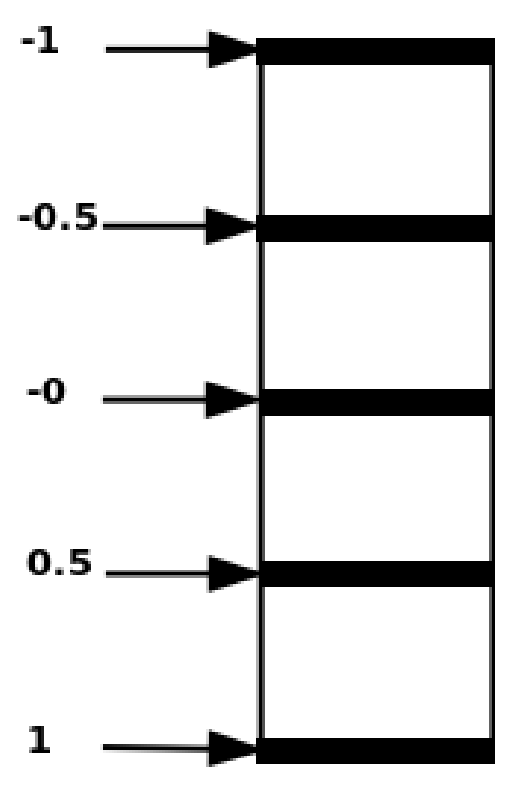
\includegraphics[width=5cm]{figuras/quatizacao.eps}
	\caption{Quantização de $s1$}
	\label{quantizacao}
\end{figure}

Isto significa que quaisquer que sejam os valores de $s1$ os mesmos devem ser convertidos para $-1$, $-0,5$, $0$, $0,5$ e $1$. 
Por exemplo, se o valor de s1 for $0,75$, será convertido para o valor $1$, se for $-0,75$ será o valor $0$ e se for $0,25$ será o valor $0,5$. À discretização dá-se o nome de resolução da CMAC.

O próximo passo é criar uma tabela para cada um dos sinais discretizados de entrada do vetor $S$.
Supondo que o vetor $S$ possui 2 sinais de entrada $s1$ e $s2$ e um número de ativações $NW*$ igual a 3, cria-se Tabela \ref{map_s1} e a Tabela \ref{map_s2}. 
Para facilitar o entendimento, irá se considerar os valores de $s1$ iguais aos inteiros de 1 até 6 e os valores de s2 iguais aos inteiros de 1 até 4.
\begin{table}[htb]
	\IBGEtab{%
		\caption{Mapeamento de $s1$}%
		\label{map_s1}
	}
	{%
		\begin{tabular}{cc}
			\toprule
			\textbf{Valores de $s1$} & \textbf{Mapeamento $m1$} \\
			\midrule
			1	&	0, 1, 2	\\
			\midrule
			2	&	3, 1, 2	\\
			\midrule
			3	&	3, 4, 3	\\
			\midrule
			4	&	3, 4, 5	\\
			\midrule
			5	&	6, 4, 6	\\
			\midrule
			6	&	6, 7, 5	\\
			\bottomrule
		\end{tabular}%
	}
	{%
		\fonte{Produzido pelo autor.}%
	}
\end{table}

\begin{table}[htb]
	\IBGEtab{%
		\caption{Mapeamento de $s2$}%
		\label{map_s2}
	}
	{%
		\begin{tabular}{cc}
			\toprule
			\textbf{Valores de $s2$} & \textbf{Mapeamento $m2$} \\
			\midrule
			1	&	0, 1, 2	\\
			\midrule
			2	&	3, 1, 2	\\
			\midrule
			3	&	3, 4, 3	\\
			\midrule
			4	&	3, 4, 5	\\
			\bottomrule
		\end{tabular}%
	}
	{%
		\fonte{Produzido pelo autor.}%
	}
\end{table}

Estas tabelas são criadas da seguinte forma:
O mapeamento consiste num número de itens igual a $NW*$, 3 no caso.
Este número é o número de pesos a serem ativados.
Para a primeira linha de cada uma das tabelas, atribui-se uma sequência de 3 valores inteiros começando com 0.
A próxima linha deve conter o próximo valor da sequência, 3, como primeiro item do mapeamento e continuar com os demais itens iguais aos da linha anterior. 
Na próxima linha, substitui-se o segundo item de mapeamento pelo próximo número da sequência, 4, mantendo-se os demais itens e assim sucessivamente.

Depois de mapeado cada valor de cada item de entrada, deve-se combinar os mapeamentos de acordo com a Tabela \ref{map_w}.
\begin{table}[htb]
	\IBGEtab{%
		\caption{Mapeamento para os pesos $W$}%
		\label{map_w}
	}
	{%
		\begin{tabular}{ccccc}
			\toprule
			\begin{tabular}{c}
				\textbf{$s2$}	\\
				\textbf{$s1$}	\\
			\end{tabular} 
			& \textbf{1} & \textbf{2} & \textbf{3} & \textbf{4} \\
			\midrule
			\textbf{1}	& 1 & 2 & 3 & 4 \\
			\bottomrule
		\end{tabular}%
	}
	{%
		\fonte{Produzido pelo autor.}%
	}
\end{table}
